\documentclass[tikz, border=10pt]{standalone}
\usepackage{pgfplots}
\pgfplotsset{compat=1.18}

\begin{document}
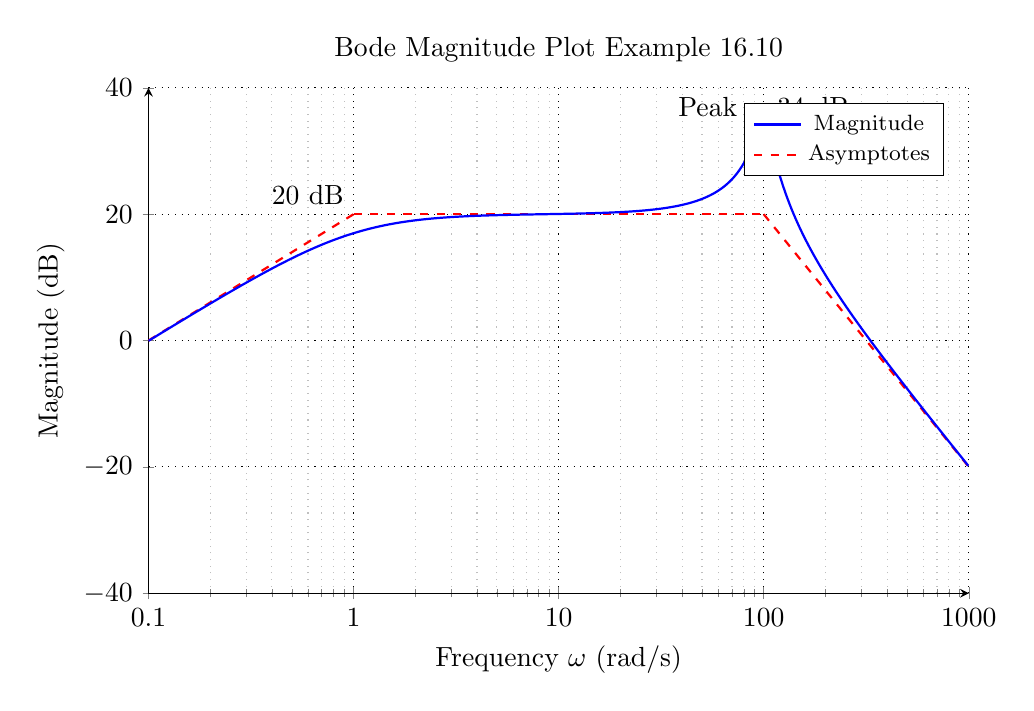
\begin{tikzpicture}
    \begin{semilogxaxis}[
        width=12cm, height=8cm,
        xlabel={Frequency $\omega$ (rad/s)},
        ylabel={Magnitude (dB)},
        xmin=0.1, xmax=1000,
        ymin=-40, ymax=40,
        grid=both,
        major grid style={dotted, black},
        minor grid style={dotted, gray!50},
        axis lines=left,
        xtick={0.1, 1, 10, 100, 1000},
        xticklabels={$0.1$, $1$, $10$, $100$, $1000$},
        legend pos=north east,
        legend style={font=\footnotesize},
        title={Bode Magnitude Plot Example 16.10}
    ]

    % Asymptotes
    % 1. Constants: 20*log10(10) = 20 dB.
    % 2. Zeros at origin: +20 dB/dec.
    % 3. Pole at w=1: -20 dB/dec.
    % 4. Double Pole at w=100: -40 dB/dec.
    
    % Net Slope:
    % w < 1: +20 dB/dec. Intercept: at w=0.1, |10s| ~ 1. 20log10(1)=0. But wait.
    % H_asymp = 10s / (1 * 1) for w small. |H| = 10w.
    % At w=0.1: |H|=1 (0 dB). At w=1: |H|=10 (20 dB).
    \draw[thick, red, dashed] (axis cs: 0.1, 0) -- (axis cs: 1, 20);
    
    % 1 < w < 100:
    % H_asymp ~= 10s / (s * 1) = 10. (20 dB).
    % Slope: +20 - 20 = 0 dB/dec.
    \draw[thick, red, dashed] (axis cs: 1, 20) -- (axis cs: 100, 20);
    
    % w > 100:
    % H_asymp ~= 10s / (s * (s/100)^2) = 10 / (s^2/10000) = 100000 / s^2.
    % At w=100: 100000/10000 = 10 (20 dB).
    % Slope: 0 - 40 = -40 dB/dec.
    % At w=1000: 100000/1000000 = 0.1 (-20 dB).
    \draw[thick, red, dashed] (axis cs: 100, 20) -- (axis cs: 1000, -20);
    
    % Actual Curve
    % |H(jw)| = 10w / ( sqrt(1+w^2) * sqrt( (1-(w/100)^2)^2 + (2*0.1*w/100)^2 ) )
    \addplot[thick, blue, domain=0.1:1000, samples=400] {20*log10( 10*x / ( sqrt(1+x^2) * sqrt( (1-(x/100)^2)^2 + (0.002*x)^2 ) ) )};
    
    \addlegendentry{Magnitude}
    \addlegendimage{thick, red, dashed}
    \addlegendentry{Asymptotes}

    % Annotations
    \node[anchor=south east] at (axis cs: 1, 20) {20 dB};
    \node[anchor=south] at (axis cs: 100, 34) {Peak $\sim$ 34 dB};
    
    % Peak calculation:
    % Correction at w=100 is +14 dB.
    % Base asymptote is 20 dB.
    % Total peak = 20 + 14 = 34 dB.

    \end{semilogxaxis}
\end{tikzpicture}
\end{document}
